\documentclass[11pt,a4paper]{ctexart}
\usepackage[margin=2.1cm]{geometry}
\usepackage{graphicx,booktabs,tabularx,longtable,float,pdflscape}
\usepackage[hidelinks]{hyperref}
\usepackage{xcolor,fancyhdr,enumitem}
\setlength{\headheight}{15pt}
\pagestyle{fancy}
\fancyhf{}
\fancyhead[L]{拾光集市——软件实现与构建}
\fancyhead[R]{实验三}
\fancyfoot[C]{\thepage}
\setlength{\parskip}{0.35em}
\renewcommand{\arraystretch}{1.3}
\setlist{nosep}
\graphicspath{{实验3_241240041_李东泽/UML/}{实验3_241240041_李东泽/验证材料/}}
\newcolumntype{Y}{>{\raggedright\arraybackslash}X}
\begin{document}
\begin{titlepage}
\centering
\vspace*{2.5cm}
{\Huge\bfseries 软件实现与构建实验报告\par}
\vspace{1.2cm}
{\LARGE 校园二手交易系统\par}
\vspace{0.5cm}
{\Large 拾光集市\par}
\vspace{2cm}
\begin{tabular}{rl}
姓名：&李东泽\\
学号：&241240041\\
项目来源：&实验一需求分析、实验二设计与建模\\
实现形式：&Python / Tkinter / SQLite 桌面应用\\
实验日期：&2026年11月10日\\
\end{tabular}
\vfill
代码、测试日志、构建产物及 UML 源文件随报告一同提交。
\end{titlepage}
\tableofcontents
\clearpage

\section{实验目的与实现范围}
本次实验将实验二的校园二手交易系统转换为可运行程序，练习 Git 本地与远程管理、构建工具的使用，以及大模型辅助开发后的检查和修正。

系统面向校园教材、数码和生活用品交易。同一普通账号可作为卖家发布商品，也可作为买家预约他人商品；管理员负责审核、举报、争议、账号与分类管理。游客无需登录即可浏览商品。程序只记录线下交付结果，不涉及支付、物流、即时聊天或第三方校园认证。

本次实现覆盖草稿、提交审核、撤回、通过、驳回、编辑重新审核、下架、预约、卖家确认或拒绝、取消申请、超时、完成与争议冻结。通知和操作日志贯穿关键操作。查询支持关键词、分类、价格区间和状态组合，统计包括商品状态、分类分布与已完成交易金额。

\section{从 UML 到代码}
\subsection{技术选择与设计调整}
实验二设计采用 Vue、Spring Boot、MySQL、Redis 和对象存储。本机已具备 Python 3.13.7，但没有 Maven；结合课程建议优先考虑桌面应用，本次将技术实现调整为 Python、Tkinter 和 SQLite。这样可用一个 Python 环境启动程序，也便于后续实验直接测试服务方法。

此次调整没有沿用原设计中的所有技术组件。登录会话和幂等结果改为关系表保存，商品图片只保存本地路径；用户角色用管理员、普通用户两个字段值表达，买家和卖家是普通用户在具体业务中的身份。数据库表保存领域实体，服务模块执行用例，避免为每张表增加只有属性的空壳类。提交目录同时保留原领域类图、商品状态图和预约时序图，另补充实际实现类图、部署图，区分需求模型与技术实现。

\subsection{模块和领域模型对应}
\begin{tabularx}{\textwidth}{p{0.22\textwidth}Y Y}
\toprule
UML对象或职责 & 实现位置 & 转换方式\\
\midrule
User、Role、Session & core.py、users/sessions表 & 注册、密码摘要、八小时会话及服务层权限\\
Product、ProductVersion & catalog.py、products/product\_versions表 & 稳定商品编号与递增版本，历史版本不可修改\\
AuditRecord、Category & catalog.py、audits/categories表 & 审核关联具体版本，停用分类不删除历史关系\\
Reservation、CancelRequest & trading.py、reservations/cancel\_requests表 & 独立预约状态与取消申请，保存标题及价格快照\\
Dispute、Report & trading.py、governance.py & 冻结交易、举报结论及恢复或取消处理\\
Notification、OperationLog & core.py、queries.py & 唯一事件键通知、追加日志及按权限查询\\
应用服务及表现层 & service.py、gui.py & 门面组合业务模块；Tkinter仅调用服务方法\\
\bottomrule
\end{tabularx}

\subsection{状态与事务规则}
商品具有 DRAFT、PENDING\_AUDIT、AUDIT\_REJECTED、PUBLISHED、RESERVED、CONFIRMED、COMPLETED、DELISTED、VIOLATION\_DELISTED、FROZEN 十种状态。草稿提交后待审核，通过才公开；修改已发布商品生成新版本并回到草稿。预约将商品从已发布转为已预约，卖家确认后转为已确认，买家确认线下交付后进入完成终态。

预约有待卖家确认、已确认、取消申请中、已取消、已拒绝、已超时、已完成、冻结八种状态。确认前可直接取消；确认后须由卖家处理取消申请，申请未处理时禁止完成。不能从完成退回已确认，不能对已下架商品预约，也不能用旧审核页面再次通过已经撤回的商品。

\begin{landscape}
\subsection{实际实现类图}
\begin{figure}[H]\centering
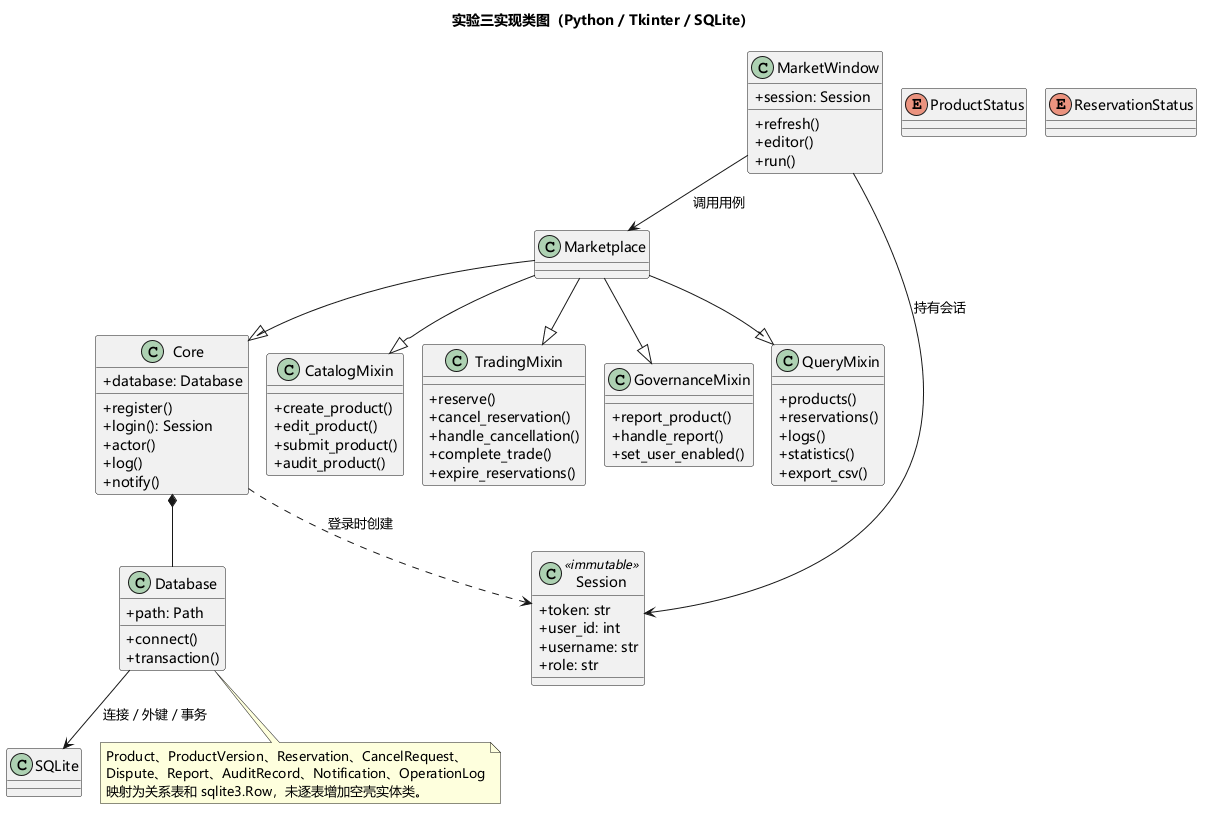
\includegraphics[width=0.95\linewidth,height=0.78\textheight,keepaspectratio]{实现类图.png}
\caption{模块化服务、桌面窗口与事务端口}
\end{figure}
\end{landscape}

\subsection{并发、异常与持久化}
所有事务命令先执行 BEGIN IMMEDIATE，取得写入事务后再读取状态并更新。SQLite 部分唯一索引限制同一商品最多存在一条有效预约，有效状态包含待确认、已确认、取消申请中和冻结。两个线程争抢同一商品时，先提交者成功，后提交者读取到已预约状态并失败；即使绕过服务方法直接插入，唯一索引仍会拒绝第二条有效预约。

重复请求按买家与请求编号查找已存在预约，同一请求重试返回原编号；同一编号改约其他商品则拒绝。价格用整数分保存，拒绝负数、零、非数值、无穷值及超过两位小数。预约保存独立价格快照，统计已完成金额使用快照而不是当前商品价格。

失败命令回滚商品、预约及通知变更，再用独立事务保存失败日志。日志只保存操作者、动作、对象、前后状态、结果、原因和时间，不写入密码或会话令牌。账号密码用随机盐与 PBKDF2-HMAC-SHA256 保存；禁用账号立即删除会话，并冻结其涉及的有效交易。恢复账号不会自动恢复冻结交易，仍需处理争议。

超时以 UTC 时间判断，满24小时未响应即失效。桌面运行时每30秒扫描，启动刷新时也补处理；可通过命令行 --sweep 独立扫描。离线期间不运行后台任务，因此不是全天候服务器调度。

\subsection{实际部署图}
\begin{figure}[H]\centering
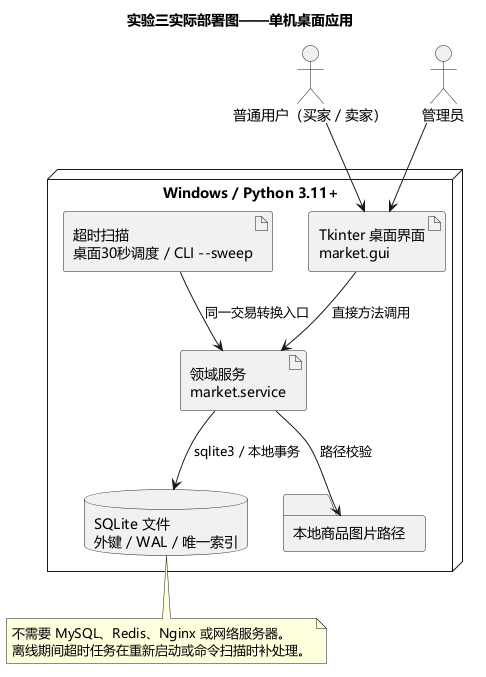
\includegraphics[width=0.93\linewidth,height=0.48\textheight,keepaspectratio]{实现部署图.png}
\caption{单机桌面应用与本地数据存储}
\end{figure}

\section{源代码规模与代码风格}
生产包共11个 Python 文件，物理行数2251行。使用 tools/verify.py 解析 AST 和 tokenize，排除空行、整行注释与模块、类、函数文档字符串后，为1951行。测试、构建脚本及自动生成的文件不计入该数值。数据库定义作为生产模块内的 SQL 字符串计入；即使另行扣除该部分，仍超过1500行。界面为手写 Tkinter 代码，没有使用 GUI 设计工具自动生成代码。

\begin{tabularx}{\textwidth}{Yrr}
\toprule 文件 & 物理行数 & 排除说明文字后\\\midrule
\texttt{\detokenize{__init__.py}} &3&1\\
\texttt{\detokenize{__main__.py}} &72&60\\
catalog.py &294&264\\
core.py &251&209\\
database.py &132&121\\
governance.py &141&128\\
gui.py &650&560\\
models.py &130&90\\
queries.py &269&240\\
service.py &11&6\\
trading.py &298&272\\\midrule
合计 &2251&1951\\\bottomrule
\end{tabularx}

风格处理采用 Ruff 格式化和 Pylint 检查。首轮发现长 SQL 字符串、bar 变量命名及多余 lambda，修正后 Pylint 输出10.00/10，退出码0。工程对参数数量、类方法数量等部分复杂度规则显式放宽，保留命名、导入、语法和常见错误检查；这些配置位于 pyproject.toml，不能把该分数理解为没有业务缺陷。

\section{辅助开发与修改过程}
本次对话式辅助工具参与了主要功能代码、测试和技术材料的生成。输入包括实验二报告、类图、状态规则、当前环境和课程交付要求。生成后直接执行检查，通过报错及运行结果修订，没有把未执行的建议当成完成证据。完整过程另存于 code/开发过程记录.md。

\begin{tabularx}{\textwidth}{p{0.15\textwidth}Y Y}
\toprule 场景 & 生成及发现的问题 & 修改与验证\\\midrule
领域实现 & 将商品、审核、预约和治理拆成模块；需处理状态竞争 & 事务检查、部分唯一索引、独立快照，并发测试验证\\
单元测试 & 初次36项测试通过，治理恢复分支仍需验证 & 增加8项回归，最终44项通过\\
风格检查 & 长SQL、多余lambda、变量命名提示 & 拆分字符串、直接传回调、重命名；Pylint退出0\\
GUI运行 & 初次截图抓到前台编辑器，不能证明应用界面 & 改按窗口句柄抓取，重新目视检查三张截图\\
构建打包 & 初次构建提示源码包缺README & 补充运行说明后重建，独立环境验证wheel\\
\bottomrule
\end{tabularx}

比较有效的输入方式是先给出状态、权限、数据约束和异常情形，再要求分模块实现与测试。例如预约不能只描述“添加预约”，还需明确重复编号、多人竞争、24小时边界和价格快照。工具适合生成规约初稿、重复结构和边界测试，但它容易把窗口截图、静态检查与实际验收混为一谈，需要用当前文件和真实运行重新核对。此报告不将自动化代码检查描述为已经由学生本人逐行审阅，后续本人核对与修订应继续保留真实 Git 提交。

\section{构建、测试与运行结果}
\subsection{构建工具与执行命令}
开发环境为 Windows 11、Python 3.13.7。使用 pyproject.toml 定义 PEP 517 构建，setuptools 为后端，build 1.6.1 为构建前端；输出源码发行包和 wheel。运行时无第三方依赖，开发检查依赖版本在 requirements-dev.txt 保存。

在 code 目录执行：
\begin{verbatim}
python -m pip install -r requirements-dev.txt
python -m pip install -e .
python tools/verify.py
python tools/gui_check.py
python -m market --db demo.db --demo
python -m market --db demo.db
\end{verbatim}

verify.py 依次统计源码、compileall 编译字节码、unittest 测试、Pylint 检查和 build 构建，任一步非零即终止。Python 不生成传统链接后的二进制程序，本次的编译结果是字节码编译成功，交付运行包是 wheel。独立虚拟环境安装 wheel 后，实际执行演示初始化、登录、查询、预约、卖家确认、买家完成及统计，证明导入的是 site-packages 安装包，而非可编辑源码路径。

\subsection{测试与运行证据}
\begin{tabularx}{\textwidth}{p{0.23\textwidth}Y}
\toprule 检查 & 实际结果与证据文件\\\midrule
源码规模 & 1951行有效生产源码；source-counts.json\\
编译 & compileall退出0；compile.txt\\
业务测试 & 44项全部通过；tests.txt，运行约30秒\\
代码风格 & Pylint 10.00/10，退出0；pylint.txt\\
构建 & wheel及tar.gz生成成功；build.txt\\
独立安装 & site-packages来源、完整交易及统计通过；installed-wheel.txt\\
桌面冒烟 & 游客、管理员、卖家页实际渲染；三张窗口截图\\
\bottomrule
\end{tabularx}

测试覆盖注册与登录、会话过期、密码轮换、非法金额、草稿可见性、越权审核、撤回后的旧审核、版本冲突、组合查询、重复预约、请求编号滥用、自己预约、并发竞争、直接数据库唯一约束、取消与完成冲突、超时、联系方式边界、举报与争议、账号禁用、日志防篡改、通知归属、CSV公式转义和数据重开持久化。测试没有证明所有 GUI 弹窗操作均正确，也没有进行大规模负载测试。

\clearpage
\subsection{实际桌面界面}
\begin{figure}[H]\centering
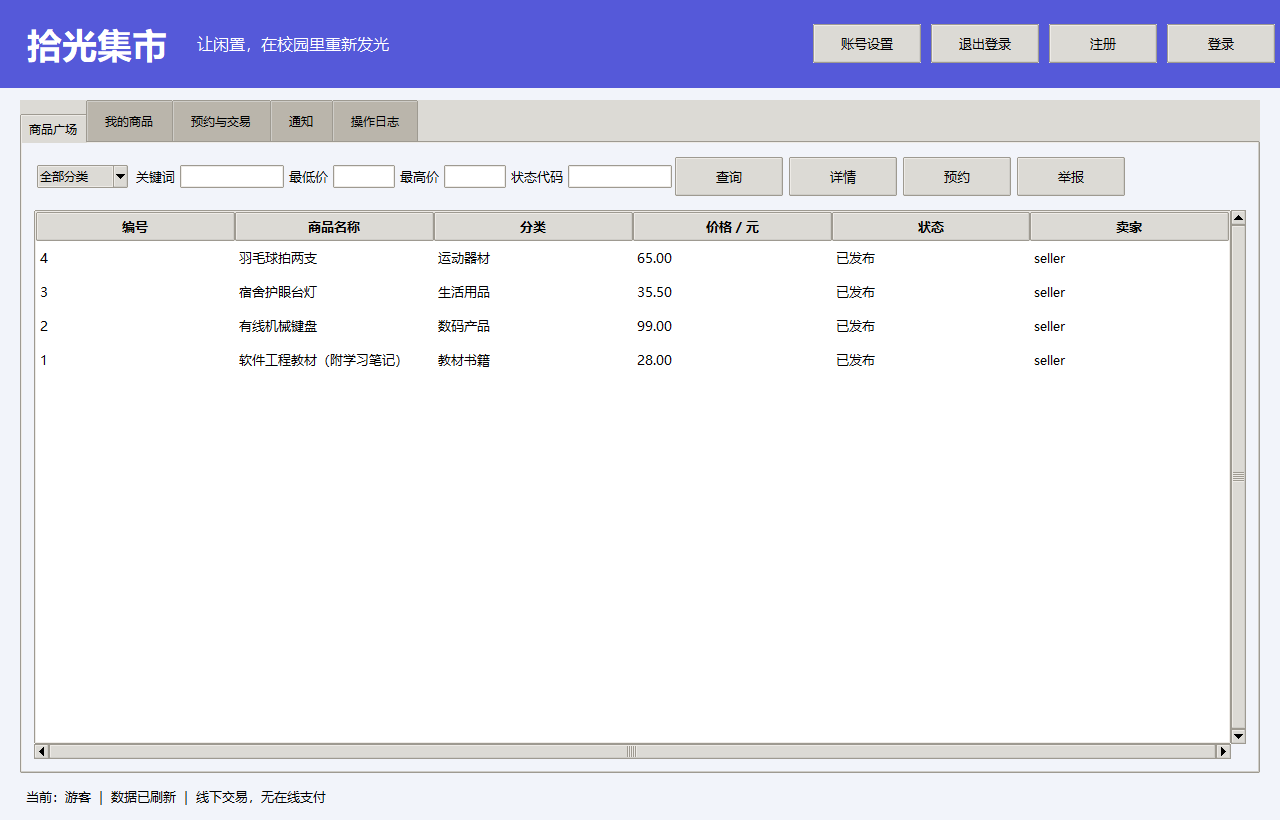
\includegraphics[width=0.98\linewidth]{01-游客商品广场.png}
\caption{游客商品查询：分类、关键词、价格和状态组合筛选}
\end{figure}
\begin{figure}[H]\centering
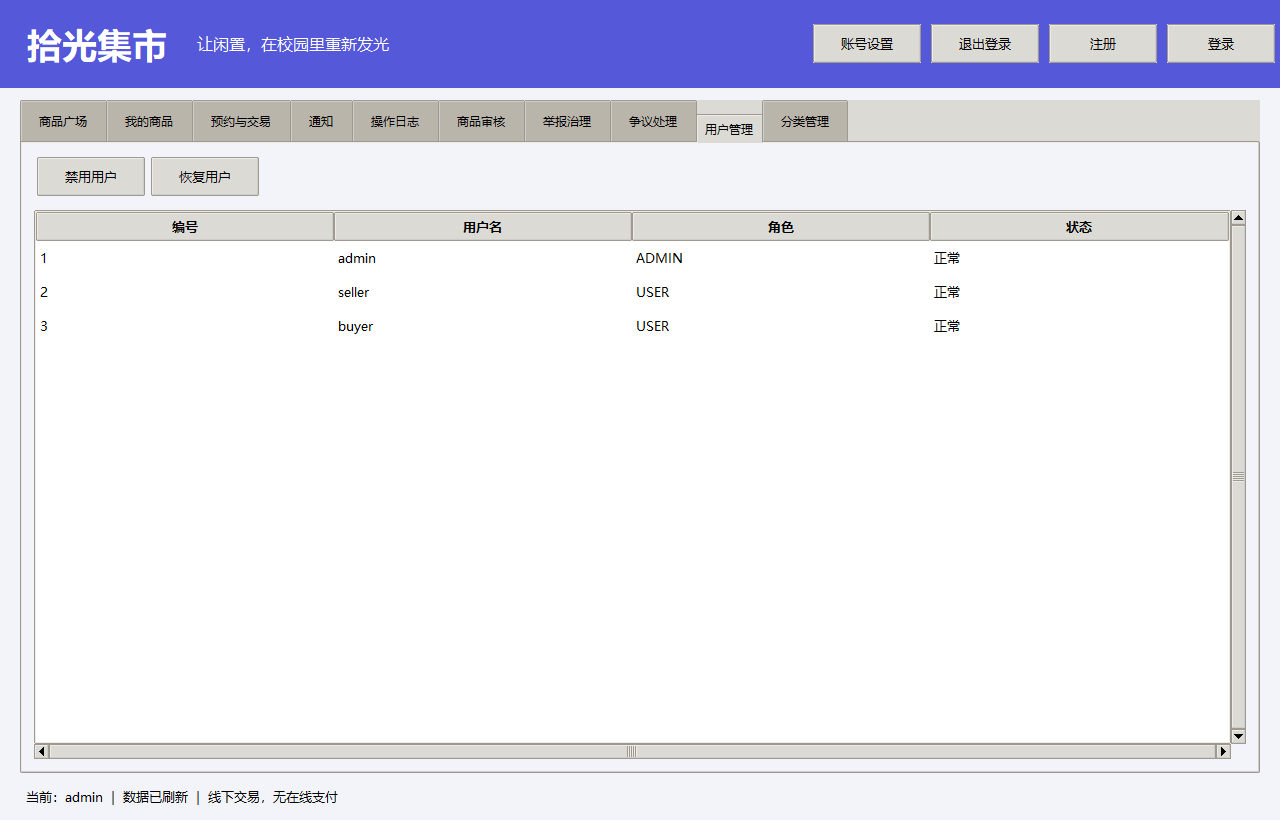
\includegraphics[width=0.98\linewidth]{02-管理员用户管理.png}
\caption{管理员后台：审核、举报、争议、用户与分类入口}
\end{figure}

\clearpage
\begin{figure}[H]\centering
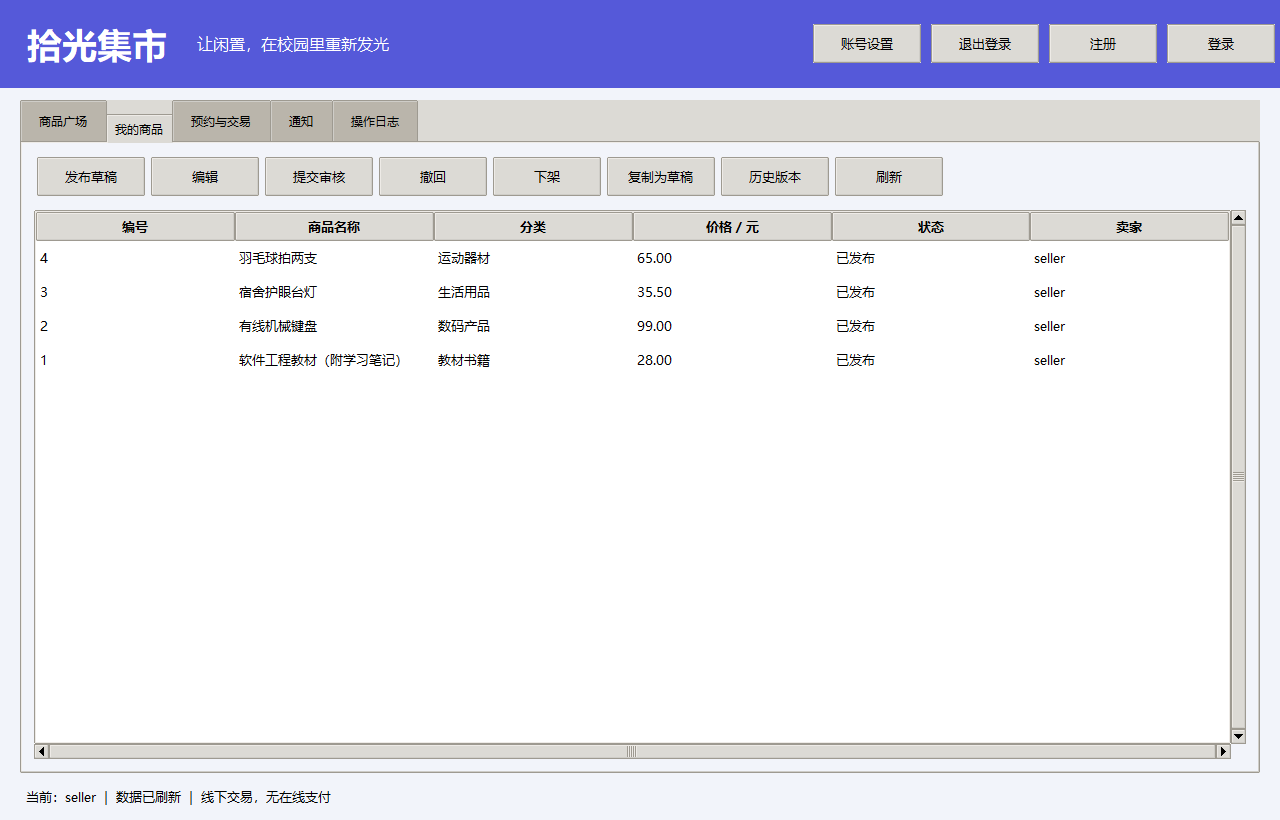
\includegraphics[width=0.98\linewidth]{03-卖家商品管理.png}
\caption{卖家商品管理：草稿、审核、撤回、下架及历史版本}
\end{figure}

\section{Git本地与远程管理}
继续使用已有仓库，实验一、实验二的提交和标签保留。仓库地址：
\url{https://github.com/Lidz-abel/software-engineering-lab1-241240041-lidongze}。
本次在 main 上形成以下真实提交：
\begin{itemize}
\item 42a2758：事务型桌面应用、主要业务与首轮测试；标签 lab3-implementation。
\item 79153f4：补充恢复与隐私回归、实现UML、构建和运行说明。
\item 最终交付提交：补充报告、验证材料与发布检查；标签 lab3-final。
\end{itemize}
开发中使用 git status 查看范围，按实验三路径暂存，避免将实验二预览文件等混入提交；使用 git diff --check 检查补丁，再提交和推送。远程地址、提交图和远端引用保存在验证材料的 git-history.txt。最终 lab3-final 指向包含本报告的交付提交，远端 main 与该标签提交核对一致。

\section{当前不足与后续安排}
当前原型适合本机演示和服务层测试。SQLite文件不提供服务器级隔离；图片只保存本地路径，迁移机器后可能失效；查询最多1000行，没有分页；超时任务在应用关闭期间需补扫。GUI详情采用字段名展示，界面可用性还有改进空间。构建与测试全部通过不能替代本人代码阅读和实际业务验收，后续实验可围绕状态覆盖、异常恢复、日志可追溯性和模块复杂度开展分析。

\section*{参考资料}
\addcontentsline{toc}{section}{参考资料}
\begin{enumerate}
\item Python官方文档：sqlite3事务、参数绑定与连接管理。\url{https://docs.python.org/3/library/sqlite3.html}
\item Python官方文档：Tkinter GUI。\url{https://docs.python.org/3/library/tkinter.html}
\item PyPA build官方用法：源码包及wheel构建。\url{https://build.pypa.io/en/latest/how-to/basic-usage.html}
\item Pylint官方文档。\url{https://pylint.readthedocs.io/}
\end{enumerate}
\end{document}
